% ----------------------------------------------------------------
% To compile make sure you use pdflatex.  Once latex is installed
% on your system, you can invoke the following command from
% the command-line.
%
% >>> pdflatex hw-template.tex
%
% A successful compilation, will produce the file hw-template.pdf.
%
%
% The remaining part of the file is preamble stuff that you don't
% have to worry about.
%
%
% Head down to where it says "Start here"
% ----------------------------------------------------------------
 
\documentclass[11pt]{article}

\usepackage{fullpage} 
\usepackage{hyperref}
\usepackage{amsmath}
\usepackage{amssymb}
\usepackage{amsthm}
\usepackage{graphicx}
\usepackage{pgf}
\usepackage{tikz}
\usetikzlibrary{arrows,automata}


\newcommand{\question}[2] {\vspace{0.3in}\noindent{\subsection*{Question #1. #2} \vspace{0.15in}}}

\renewcommand{\part}[1] {{\vspace{0.15in}\noindent\textbf (#1)} \vspace{0.10in}}



%  ----------------------------------------------------------------
%                         Start here
% ----------------------------------------------------------------
 
\begin{document}

\title{Assignment \#X} %Replace X with the appropriate number
\author{\Large Jane Doe\\ %Replace with your name
CSCE 433: Formal Languages and Automata} %If necessary, replace with your course number and title
\date{\today} 

\maketitle


\question{1}{Mathematical Symbols}

This is an example of an answer to a homework question.  In your answer, you may incorporate a variety of mathematical symbols:
\smallskip 

\begin{itemize}
\item Fractions: $\frac{2}{3}, \frac{n}{10}, \frac{x^2 + x + 5}{x - 10}$
\item Binomial coefficients: ${5 \choose 2} = 10$
\item Subscripts and superscripts: $t_0$, $t^2$, $t_0^{2 \over 3}$, 
\item Greek letters: $\alpha$, $\beta$, $\delta$, $\gamma$, $\lambda$, $\pi$.
\item Summations: $\sum_{i=1}^n i = \frac{n(n+1)}{2}$.
\end{itemize}


\question{2}{Proving Gauss's Formula by Mathematical Induction}

This is another example of a question.  In this case, it's a multi-part question.

\part{a} Consider \textit{Gauss's formula}:

% equations are automatically centered!
\begin{eqnarray}
\sum_{i=1}^n i = {{n(n+1)} \over 2}  % as usual, liberal use of curly braces...
\label{gauss}        % labelled so we can refer to this formula by number
\end{eqnarray}

\part{b} 

\begin{proof}
We will prove equation \ref{gauss} by mathematical induction.

\begin{itemize}
\item \textit{\underline{Base case}}: If $n = 1$, then $1 = \frac{1(2)}{2} =1$. Base case holds.

\item \textit{\underline{Inductive hypothesis}}: Assume the equation holds for $2 \leq n \leq k$.

\item \textit{\underline{Inductive step}}: For $n = k+1$, we have
\begin{equation*}
\begin{aligned}    % the star suppresses the equation numbers 
\sum_{i=1}^{k+1} i &= (k+1) + \sum_{i=1}^k i & \\
                   &= (k+1) + \frac{k(k+1)}{2} & \textup{(by inductive hypothesis)} \\    
                   &= {{2k+2 + k(k+1)} \over 2} &\\
                   &= {{k^2 + 3k + 2} \over 2}&\\
                   &= {{(k+1)(k+2)} \over 2} &
\end{aligned}
% notice \\ to indicate newline and the &=& to line up the equals signs 
\end{equation*}
\end{itemize}

The last line shows that for $n = k+1$, Gauss'
formula still holds! We've shown that the formula holds
for $n=1$. And, we've shown that if it holds for $n=k$, it must hold for $n=k+1$. Therefore, the equation must hold for all $n$. $\qedhere$ 

\end{proof}



\question{3}{Constructing DFA's}

\part{a} Design a DFA to accept the language $L = \{w:\text{$w$ is a binary string containing the substring 01}\}$.

\begin{figure}[h]
\centering
\fbox{
  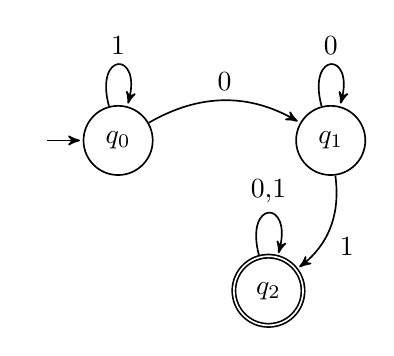
\begin{tikzpicture}[->,>=stealth',shorten >=1pt,auto,node distance=2.7cm, semithick, initial text={}]
  
  \tikzstyle{every state}=[fill=white,draw=black,text=black]

  \node[initial,state]    (0)                    {$q_0$};
  \node[state]            (1) [right of=0] {$q_1$};
  \node[accepting, state] (2) [below right of=0] {$q_2$};
 ;

  \path (0) edge [bend left]  node {0} (1)
            edge [loop above] node {1} (0)
        
        (1) edge [bend left]  node {1} (2)
            edge [loop above] node {0} (1)
        
        (2) edge  [loop above] node {0,1} (2)             
 ;                      
  \end{tikzpicture}
}
\caption{A DFA $M$ that accepts the language $L$. The diagram was drawn using the \texttt{automata} library for the \texttt{tikz} package.}
\end{figure}

\part{b} The formal specification of DFA $M = (Q, \Sigma, \delta, q, F)$, where
\begin{itemize}
	\item $Q = \{q_0, q_1, q_2\}$, 	
	\item $\Sigma = \{0,1\}$,
	\item $q = q_0$,
	\item $F = \{q_2\}$, and
	\item $\delta$ is defined as follows. \\

\begin{tabular}{|c||c|c|}  \hline
      & 0 & 1 \\ \hline 
$q_0$ & $q_1$ & $q_0$ \\ \hline 
$q_1$ & $q_1$ & $q_2$ \\ \hline
$q_2$ & $q_2$ & $q_2$ \\ \hline 
\end{tabular}

	
\end{itemize}


\part{c} You may hand-draw your figures as long as they are readable and in a format (e.g., pdf, jpg) that \LaTeX\ can handle.
\begin{figure}[h]
\centering 
\fbox{
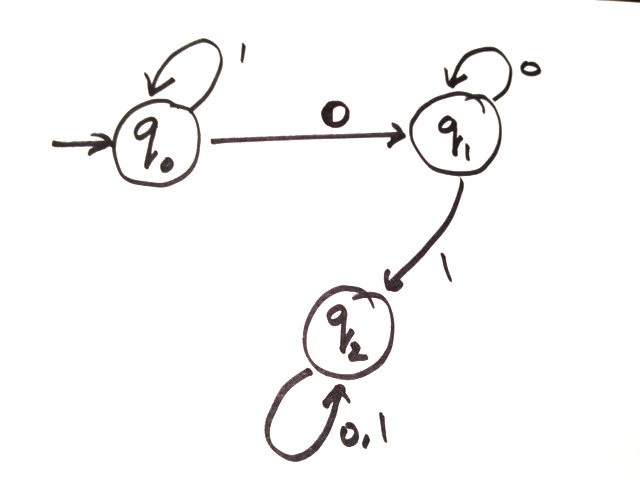
\includegraphics[scale=0.3]{hand-drawn-dfa.jpg}
}
\caption{A hand-drawn DFA included into \LaTeX\ as a JPG image.}	
\end{figure}





\end{document}

